\documentclass{article} % For LaTeX2e
\usepackage{iclr2017_conference,times}
\usepackage{hyperref}
\usepackage{url}

\usepackage[T1]{fontenc}
\usepackage[utf8]{inputenc}
\usepackage[francais]{babel}

\usepackage{amsmath}
\usepackage{amssymb}
\usepackage{graphicx}

\usepackage{algorithm}
\usepackage{algorithmic}


\title{Toward predictive machine learning for active vision}


\author{Anonymous
%Emmanuel Daucé \\
%Ecole Centrale de Marseille, Aix Marseille Univ, Inserm \\
%INS, Institut de Neurosciences des Systèmes\\ 
%Marseille, France\\
%\texttt{emmanuel.dauce@centrale-marseille.fr} \\
}

% The \author macro works with any number of authors. There are two commands
% used to separate the names and addresses of multiple authors: \And and \AND.
%
% Using \And between authors leaves it to \LaTeX{} to determine where to break
% the lines. Using \AND forces a linebreak at that point. So, if \LaTeX{}
% puts 3 of 4 authors names on the first line, and the last on the second
% line, try using \AND instead of \And before the third author name.

\newcommand{\fix}{\marginpar{FIX}}
\newcommand{\new}{\marginpar{NEW}}

%\iclrfinalcopy % Uncomment for camera-ready version

\begin{document}


\maketitle

\begin{abstract}
We develop a comprehensive description of the active inference framework, as proposed by \cite{friston2010free}, under a machine-learning compliant perspective. Stemming from a biological inspiration and the auto-encoding principles, a sketch of a cognitive architecture is proposed that should provide ways to implement \emph{estimation-oriented} control policies under a POMDP perspective. 
Computer simulations illustrate the effectiveness of the approach through a foveated inspection of the input data.
The pros and cons of the control policy are reviewed in details, showing interesting promises in term of processing compression, but also putative risks of a confirmation bias that may degrade the recognition performance if the model is too optimistic about its own predictions. The presented formalism is fully compliant with the auto-encoding framework and would deserve further developments under variational encoding architectures.
\end{abstract}

\section{Motivation}

	The oculo-motor activity is an essential component of man and animal behavior, subserving most of daily displacements and interactions with objects, devices or people. By moving gaze with the eyes, the center of sight is constantly and actively moving around during all waking time.  %Though taking a large part in brain activity, the principles underlying those visually guided movements are still a subject of debate in neurosciences.
	%The most documented case of active perception is gaze orientation, primarily studied in both man and animal \cite{yarbus1967eye,robinson1968eye}. A nice review of principal promises of \emph{animate} vision against passive vision  is presented in \cite{ballard1991animate},  in relation with eye-hand coordination in computer vision.
	%A salient feature of superior vertebrates visual apparatus is the foveated retina that concentrates  photoreceptors over a small central portion of the visual field.
	%, {\color{magenta} following an approximate exponential decrease of resolution from the center to the periphery [REF?]}. 
	The scanning of the visual scene is principally done with high-speed targeted eye movements called saccades (\cite{yarbus1967eye}), that sequentially capture local chunks of the visual scene. 
	Though ubiquitous in biology, object recognition through saccades is seldom considered in artificial vision. The reasons are many, of which the existence of high-performance sensors that provide millions of pixels at low cost. %\footnote{in contrast with animals retina whose actual design relies on a long optimization process under severe resource constraints.}.
	Increasingly powerful computing devices are then assigned to compute in parallel those millions of pixels to perform recognition, consuming resources in a brute-force fashion. 
	
	The example of animal vision encourages however a different approach towards more parsimonious recognition algorithms. A salient aspect of animal vision is thus the use of \emph{active} sensing devices, capable of moving around under some degrees of freedom in order to choose a particular viewpoint. The existence of a set of possible sensor movements calls for the development of specific algorithms that should \emph{solve the viewpoint selection problem}. A computer vision program should for instance look back from past experience to see which viewpoint to use to provide the most useful information about a scene. Optimizing the sensor displacements across time may then be a part of computer vision algorithms, in combination with traditional pixel-based operations. 
	
	More generally, the idea of viewpoints selection turns out to consider beforehand the computations that need to be done to achieve a certain task. A virtual sensing device should for instance act like a filter that would select which part of the signal should be worth considering, and which part should be bypassed.  
	This may be the case for robots and drones  that need to react fast with light and low-power sensing devices. Similarly, in computer vision, Mega-pixel high-resolution images appeals for selective convolution over the images, in order to avoid unnecessary matrix products. Less intuitively, the ever-growing  learning databases used in machine learning also suggest an intelligent scanning of the data, in a way that should retain only the critical examples or features, depending on context, before performing learning on it.  
	Behind the viewpoint selection problem thus lies a feature selection problem, which should rely on a context. 
	%An evolving context over time would imply a changing feature selection. 
	%To put it clear, the visual features (or viewpoints) that should be used to recognize an armchair should not  be the same as the ones used to recognize a squirrel. If you are in a park, and there is a good chance to meet a squirrel, you should probably look around in the trees for something small and furry, whereas if you enter in a hotel, where there is a good chance to find an armchair, you may look sideways for something large and static, so you can ignore the "up in the tree" viewpoint and the small and furry features, in your computations, to confirm your hypothesis.
	
	
	
	%\subsection{Gaze orientation in biology}
	
	
	
	%\subsection{Active vision and active inference}	
	
	The concept of active vision and/or active perception is present in robotic literature under different acceptances. In \cite{aloimonos1988active}, the authors address the case of multi-view image processing of a scene, i.e. show that some ill-posed object recognition problems become well-posed as soon as several views on the  same object are considered. The term was also proposed in \cite{bajcsy1988active} as a roadmap for the development of artificial vision systems, that provides a first interpretation of active vision in the terms of sequential Bayesian estimation, further developed in \cite{najemnik2005optimal,butko2010infomax,ahmad2013active,potthast2016active}.
	
The active inference paradigm was independently introduced in neuroscience through the work of ~\cite{friston2010free,friston2012perceptions}. % 
The general setup proposed by Friston and colleagues is that of a general tendency of the brain to counteract surprising and unpredictible sensory events through building generative models that improve their predictions over time and render the world more amenable. This improvement is mainly done through sampling the environment and extracting statistical invariants that are used in return to predict upcoming events.
Building a model thus rests on extracting a repertoire of invariants and organizing them so as to process the incoming sensory data efficiently through predictive coding (see \cite{rao1999predictive}). This proposition, gathered under the ``Variational Free Energy Minimization'' umbrella, is reminiscent of the auto-encoding theory proposed by \cite{hinton1994autoencoders}, but introduces a new perspective on coding
for \emph{it formally links dictionary construction from data and (optimal) motor control}.
In particular, motor control is here considered as a particular implementation of a \emph{sampling process}, that is at the core of the estimation of a complex posterior distribution. 

%The active inference approach relies on a longstanding history of probabilistic modelling in signal processing and control (\cite{Kalman1960,Baum1966,friston1994statistical}).  Put formally, the physical world  takes the form of a generative process $p$ that is the cause of the sensory stream. This process is not visible in itself but is only sensed through a (non reliable) measure process that provides an observation vector $x$. The inference problem consists in estimating the underlying causes of the observation, that rests on a latent state vector $z$ and a control $u$.  Then, the evolution of $x$ relies on both $u$ and $z$ in the form of a stochastic dynamical system undergoing an external forcing command $u$, i.e. :
%\begin{align}
%\dot{z} &= A(z) + B(u) + \text{process noise}\label{eq:kalman-process}\\
%x &= C(z) + D(u) + \text{measurement noise} \label{eq:kalman-measure}
%\end{align}  
%where $A$, $B$, $C$ and $D$ constitute a generative model $p(x,u,z,\dot{z})$ that explicits the dependencies between $u$, $x$ and $z$. % \footnote{We note for simplicity $p(x,u,z)$ in the following, with each variable counting for its state vector and possible higher moments.}. 
%The calculation of $\dot{z}$ from $z$ and $u$ and the calculation of $z$ from $u$ and $x$ rely on a model $p = \{A,B,C,D,\text{noise models}\}$. The model can then be inverted in order to compensate for the drift of the state estimate \cite{Kalman1960,Baum1966}. The more accurate the model, the better this estimation. 

\section{Perception-driven control}
The active inference relies on a longstanding history of probabilistic modelling in signal processing and control (\cite{Kalman1960,Baum1966,friston1994statistical}).  Put formally, the physical world  takes the form of a generative process $P$ that is the cause of the sensory stream. This process is not visible in itself but is only sensed through a (non reliable) measure process that provides an observation vector $\boldsymbol{x}$. The inference problem consists in estimating the underlying causes of the observation, that rests on a latent state vector $\boldsymbol{z}$ and a control $\boldsymbol{u}$. 
The question addressed by \cite{friston2012perceptions} is the design a \emph{controller} \emph{that outputs a control $\boldsymbol{u}$ from $\boldsymbol{z}$} so as to maximize the accuracy of this state estimation process. This is the purpose of a \emph{perception-driven} controller.

The logic behind the model is that of an external sensory scene $\mathcal{X}$ that is never disclosed in full, but only sensed under a particular view $\boldsymbol{x}$ under sensor orientation $\boldsymbol{u}$ (like it is the case in foveated vision). 
%We moreover consider an organization of the visual scene in objects (or causes), whose presence and position is continuously checked by visual inspection. The objects may be described by their identity $o$ and position in space $s$, but for simplicity $o$ and $s$ are here reduced to a single variable $z = (o, s)$. 
Knowing that $\boldsymbol{z}$ is invariant to changing the sensor position $\boldsymbol{u}$, uncovering $\boldsymbol{z}$ should rest on
collecting sensory patches $\boldsymbol{x}$'s through changing $\boldsymbol{u}$ (sensor orientation) across time in order to refine $\boldsymbol{z}$'s estimation. 
Considering now that a certain prior $\rho_0
(\boldsymbol{z})$ has been formed about $\boldsymbol{z}$, choosing  $\boldsymbol{u}$ conducts the sight in a region of the visual field that provides $\boldsymbol{x}$, which in turn allows to refine the estimation of $\boldsymbol{z}$.
Each saccade should consolidate a running assumption about $\boldsymbol{z}$ (scene constituents), that may be retained and propagated from step to step, until enough evidence is gathered.

Instead of choosing $\boldsymbol{u}$ at random, the general objective of an \emph{active inference} framework is to choose $\boldsymbol{u}$ in a way that should minimize \emph{at most} the current uncertainty about $\boldsymbol{z}$. 
The knowledge about $\boldsymbol{z}$ can be reflected in a posterior distribution $\rho(\boldsymbol{z})$ . The better the knowledge (precision) about a sensory scene, the lower the \emph{entropy} of $\rho$, with:
\begin{equation}
H(\rho) = E_{\boldsymbol{z}\sim \rho}[- \log \rho(\boldsymbol{z})]\label{eq:entropy}
\end{equation}

It is shown in \cite{friston2012perceptions} that minimizing the entropy of the posterior through action can be linked to minimizing the variational free energy attached to the sensory scene. 
%$ P(z|u,y) \propto P(y|z,u) \pi(z)$. 
%One needs thus to choose $u$ appropriately in order to reduce the uncertainty about $z$, given the actual $y$, i.e minimize the entropy :
%$u^* = \underset{u \in \mathcal{U}}{\text{argmin }} H$ with $H = E(-\log P(z|u,y))$.
The control $\boldsymbol{u}$ is thus expected to reduce at most the entropy of $\rho$ at each step. This optimal $\boldsymbol{u}$ is not known in advance, because $\boldsymbol{x}$ is only read \emph{after} $\boldsymbol{u}$ has been carried out. Then comes the predictive framework that identifies the effect of $\boldsymbol{u}$ with its most probable outcome, according to a \emph{generative} model $P$.
	
If we take a step back, the general formulation of the generative model is that of a feedback control framework, under a discrete Bayesian inference formalism. %given a generative model $p$, and an initial condition $z_0$ (or initial guess), a control $u \in \mathcal{U}$ allows to make a \emph{prediction} about a forthcoming $z$, which allows in turn to make a prediction about the forthcoming $x$. Those 
Given an initial state $\boldsymbol{z}_0$, the prediction rests on two conditional distributions, namely $P(\boldsymbol{z}|\boldsymbol{u},\boldsymbol{z}_0)$ --~the link dynamics that generates $\boldsymbol{z}$~-- and $P(\boldsymbol{x}|\boldsymbol{z},\boldsymbol{u})$ --~the measure process that generates $\boldsymbol{x}$~--. % (the discrete analog of (\ref{eq:kalman-process}) and (\ref{eq:kalman-measure})). %, which allows to predict the next $p(x,z|u,z_0) = p(x|z,u) p(z|u,z_0) = p(z|x,u,z_0)p(x|u,z_0)$.
Then, the forthcoming posterior distribution is (Bayes rule):
	\begin{align}
	P(\boldsymbol{z}|\boldsymbol{x},\boldsymbol{u},\boldsymbol{z}_0) &= \frac{P(\boldsymbol{x},\boldsymbol{z}|\boldsymbol{u},\boldsymbol{z}_0)}{P(\boldsymbol{x}|\boldsymbol{u},\boldsymbol{z}_0)}
	= \frac{P(\boldsymbol{x}|\boldsymbol{z},\boldsymbol{u}) P(\boldsymbol{z}|\boldsymbol{u},\boldsymbol{z}_0)}{\sum_{\boldsymbol{z}'}P(\boldsymbol{x}|\boldsymbol{z}',\boldsymbol{u}) P(\boldsymbol{z}'|\boldsymbol{u},\boldsymbol{z}_0)}\label{eq:post}
	\end{align}
	
	so that the forthcoming entropy expectation is:
	\begin{align}
	E_{\boldsymbol{x}}\left[H(\rho)|_{\boldsymbol{x}, \boldsymbol{u}, \boldsymbol{z}_0}\right] &=  E_{\boldsymbol{x}}\left[E_{\boldsymbol{z}}\left[-\log  P(\boldsymbol{z}|\boldsymbol{x},\boldsymbol{u},\boldsymbol{z}_0)\right]\right]
	\end{align}
	and the optimal $\boldsymbol{u}$ is:
	\begin{align}
	\hat{\boldsymbol{u}} &= \underset{\boldsymbol{u} \in \mathcal{U}}{\text{argmin }} E_{\boldsymbol{x}}\left[H(\rho)|_{\boldsymbol{x}, \boldsymbol{u}, \boldsymbol{z}_0}\right]
	\end{align}
	%with:
	%\begin{align}
	%q(\boldsymbol{z})|_{\boldsymbol{u},\boldsymbol{z}_0} &= \int P(\boldsymbol{z}|\boldsymbol{x},\boldsymbol{u},\boldsymbol{z}_0)P(\boldsymbol{x}) d\boldsymbol{x}
	%\end{align}
	
	In practice, the analytic calculations are out of reach (in particular for predicting the next sensory field $\boldsymbol{x}$).  One thus need to consider an \emph{estimate} $\tilde{\boldsymbol{u}} \simeq \hat{\boldsymbol{u}}$ that should rely on sampling from the generative process $P$ to 
	predict the effect of $\boldsymbol{u}$,  i.e. 
	\begin{align} \tilde{\boldsymbol{u}} = \underset{\boldsymbol{u}}{\text{argmin}} \frac{1}{N} \sum_{\substack{i = 1..N\\ \boldsymbol{x}^{(i)} \sim P(.|\boldsymbol{u}, \boldsymbol{z}_0)\\ \boldsymbol{z}^{(i)} \sim P(.|\boldsymbol{x}^{(i)}, \boldsymbol{u}, \boldsymbol{z}_0)}} -\log P(\boldsymbol{z}^{(i)}| \boldsymbol{x}^{(i)}, \boldsymbol{u}, \boldsymbol{z}_0) \label{eq:MC} \end{align} or on an even sharper direct estimation through maximum likelihood estimates (point estimate):
	\begin{align}
	&\tilde{\boldsymbol{x}}_{\boldsymbol{u}} = \underset{\boldsymbol{x}}{\text{argmax }} P(\boldsymbol{x}|\boldsymbol{u}, \boldsymbol{z}_0) \label{eq:step-1}\\	
	&\tilde{\boldsymbol{z}}_{\boldsymbol{u}} = \underset{\boldsymbol{z}}{\text{argmax }} P(\boldsymbol{z}|\tilde{\boldsymbol{x}}_{\boldsymbol{u}}, \boldsymbol{u}, \boldsymbol{z}_0) \label{eq:step-2}\\
	&\tilde{\boldsymbol{u}} = \underset{\boldsymbol{u}}{\text{argmin }} - \log P(\tilde{\boldsymbol{z}}_{\boldsymbol{u}}|\tilde{\boldsymbol{x}}_{\boldsymbol{u}}, \boldsymbol{u}, \boldsymbol{z}_0)	\label{eq:step-3}
	\end{align}


This operation can be repeated in a sequence, where the actual control $\boldsymbol{u} = \tilde{\boldsymbol{u}}$ is followed by reading the actual visual field $\boldsymbol{x}$, which in turn allows to update the actual posterior distribution over the $\boldsymbol{z}$'s. This updated posterior becomes the prior of the next decision step, i.e. $\boldsymbol{z}_0'\sim  P(\boldsymbol{z}|\boldsymbol{x}, \boldsymbol{u}, \boldsymbol{z}_0)$ so that a new control $\boldsymbol{u}'$ can be carried out, etc. 

If we denote $T$ the final step of the process,  with $\boldsymbol{u}_{0:T-1}$ the actual sequence of controls and $\boldsymbol{x}_{1:T}$ the actual sequence of observations, the final posterior estimate becomes $P(\boldsymbol{z}_{1:T}|\boldsymbol{z}_0, \boldsymbol{u}_{0:T-1}, \boldsymbol{x}_{1:T})$, which complies with a Partially Observed Markov Decision Process (POMDP) estimation (see fig.~\ref{fig:graphical}), whose policy would be defined by the entropy minimization principles defined above, precisely to facilitate the estimation process. The active inference framework thus appears  as a \emph{scene understanding oriented policy} (it has no other purpose than facilitate estimation).

\begin{figure}[t!]
	\centerline{
		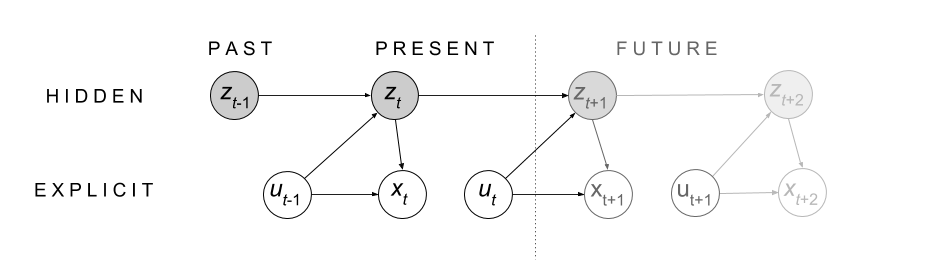
\includegraphics[width = \linewidth]{img/ICLR-graphical-v2.png} 
	}
	\caption{Graphical model (see text)}\label{fig:graphical}
\end{figure}

%If we now turn back to the active vision analogy, $q(z_t)$ is the current assumption about the visual scene under exploration, which is used as a context ("I'm in a park with many squirrels around" --~$z_t$~--) to form a prediction ("If I look up, ..." --~$u_t$~-- "I may see a squirrel" --~$\tilde{x}_{t+1}$~--~) which would reduce the entropy of the posterior $q(z_{t+1})$ for it would reduce the uncertainty about the constituents of the scene.  This incites me to look up (rather than looking down the grass) so that I can effectively process $x_{t+1}$, which may result in improving (or not) the entropy of the posterior depending on whether my prediction was correct or not. I may then look to other places up around to precisely locate squirrels, but I probably don't need to inspect the grass or the lake for the same purpose, so I can currently avoid spending time looking there.   

The active perception framework allows many relieving simplification from the general POMDP estimation framework, first in considering that changing $\boldsymbol{u}$ has no effect on the scene constituents, i.e. $P(\boldsymbol{z}_{t+1}|\boldsymbol{u},\boldsymbol{z}_t) = P(\boldsymbol{z}_{t+1}|\boldsymbol{z}_t)$. Then using the \emph{static} assumption, that considers that no significant change should take place in the scene during a saccadic exploration process, i.e. $\forall t, t', \boldsymbol{z}_{t} = \boldsymbol{z}_{t'} = \boldsymbol{z}$. This finally entails a simplified chaining of the posterior estimation:
 	\begin{align}
 	P(\boldsymbol{z}|\boldsymbol{z}_0,\boldsymbol{x}_{1:t+1},\boldsymbol{u}_{0:t}) &= \frac{P(\boldsymbol{x}_{t+1}|\boldsymbol{z},\boldsymbol{u}_t) P(\boldsymbol{z}|\boldsymbol{z}_0,\boldsymbol{x}_{1:t}, \boldsymbol{u}_{0:t-1})}{\sum_{\boldsymbol{z}'}P(\boldsymbol{x}_{t+1}|\boldsymbol{z}',\boldsymbol{u}_t) P(\boldsymbol{z}'|\boldsymbol{z}_0,\boldsymbol{x}_{1:t}, \boldsymbol{u}_{0:t-1})}
 	\end{align}
issuing a final estimate $P(\boldsymbol{z}|\boldsymbol{z}_0, \boldsymbol{x}_{1:T}, \boldsymbol{u}_{0:T-1})$.  


%{\color{blue} Put in a sequential setup :
%	\begin{align*}
%	&\tilde{u}_{1:T} = \underset{u_{1:T}}{\text{argmin }} - \log p(z^\text{max}_{1:T}|x^\text{max}_{1:T}, u_{1:T}, z_0)	\\
			%	&z^\text{max}_{1:T} = \underset{z_{1:T}}{\text{argmax }} p(z_{1:T}|x^\text{max}_{1:T}, u_{1:T}, z_0)\\
%	&x^\text{max}_{1:T} = \underset{x_{1:T}}{\text{argmax }} p(x_{1:T}|u_{1:T},z_0)
%	\end{align*}
%	}

\section{Interpretation}

The active inference framework, that is rooted on the auto-encoding theory (Free Energy minimization) and predictive coding, provides a clear roadmap toward an effective implementation in artificial devices. It should rely on four elements, namely:
\begin{itemize}
	\item a \emph{generative model} $p$ that should predict the next sensory scene $\boldsymbol{x}$ under the current hypothesis $\boldsymbol{z}$ and viewpoint $\boldsymbol{u}$, 
$$p(\boldsymbol{x}|\boldsymbol{u}, \boldsymbol{z}_0) \simeq \sum_{\boldsymbol{z}'}P(\boldsymbol{x}|\boldsymbol{z}',\boldsymbol{u}) P(\boldsymbol{z}'|\boldsymbol{u},\boldsymbol{z}_0) $$
   \item an \emph{inference model} $q$ that should predict the next posterior $\boldsymbol{z}$ under putative observation $\tilde{\boldsymbol{x}}$ and viewpoint $\boldsymbol{u}$, i.e.
$$q(\boldsymbol{z}|\tilde{\boldsymbol{x}}, \boldsymbol{u},\boldsymbol{z}_0) \simeq  P(\boldsymbol{z}|\tilde{\boldsymbol{x}}, \boldsymbol{u},\boldsymbol{z}_0) \text{\hspace{.2cm}---~see eq.~(\ref{eq:post})~---}$$  %\sum_{\boldsymbol{z}_0'} P(\boldsymbol{z} |\boldsymbol{x}, \boldsymbol{u}, \boldsymbol{z}_0')  P(\boldsymbol{z}_0')$$
(with $\boldsymbol{z}_0$ a shortcut for the previous estimate in an estimation sequence and the link dynamics $P(\boldsymbol{z}|\boldsymbol{u},\boldsymbol{z}_0)$ implicitly embedded in both the generative and inference models),
\item and a policy $\pi$ that should use a "two-steps ahead prediction" principle (next view prediction first and then inference on predicted view) to issue an optimal control $\boldsymbol{u}$ according to either eq.~(\ref{eq:MC}) or eqs.~(\ref{eq:step-1}--\ref{eq:step-3})
\end{itemize}  
%The graphical model shown in figure \ref{fig:graphical} entails a generative 
%and an inference 
%networks .
%Those networks should be learned aside in an unsupervised way using auto-encoding architectures, for giving support to the scene exploration policy  to issue a control. 

%It must be noticed that the generative model (eqs \ref{eq:step-1}-\ref{eq:step-2}) stems from the present $z_t$ and present $u_t$ while the inference model (2) heads toward the future $z_{t+1}$.  In the case of active vision however, we assume that $z_t = z_{t+1}$ (steady-state assumption~--~see previous section) so that the generative and inference models may be learned over the same encoding. The upper arrow represents the fact that the memory of the previous state participates in the present state estimate, and the dashed arrow represents the control policy, that is not inferred but optimized from two steps ahead predictions.

Under the computer vision perspective, and considering $\boldsymbol{z}_0 = \boldsymbol{z}$ (static scene assumption), each different $\boldsymbol{u}$ corresponds to a different viewpoint over a static image, with a set of generative
$ \left\{p_{\boldsymbol{u}}(\boldsymbol{x}|\boldsymbol{z})\right\}_{\boldsymbol{u}\in\mathcal{U}}$
and inference
$ \left\{q_{\boldsymbol{u}}(\boldsymbol{z}|\boldsymbol{x})\right\}_{\boldsymbol{u}\in\mathcal{U}}$ 
%(with $\boldsymbol{z}$ equal to $\boldsymbol{z}_0$), 
models learned systematically for each different viewpoint $\boldsymbol{u}$. The idea of having many models to identify a scene complies with the weak classifiers evidence accumulation principle used in \cite{viola2003fast}. In image processing, the weak classifiers generally reduce to a set of low-level filters, with $\boldsymbol{u}$ corresponding to the image coordinates at which the filters are applied. They may also correspond to the first layer of convolution filters used in convolutional neural networks. Under that perspective, choosing $\boldsymbol{u}$ (or choosing a subset of $\boldsymbol{u}$'s) corresponds to choosing the set of coordinates at which the filter is applied, with each image patch obtained from a particular coordinate corresponding to a "viewpoint" over the whole image (like looking in a keyhole). 

The active inference perspective also addresses important aspects of representation learning, for the scene encoding $\boldsymbol{z}$ is learned as an invariant over many viewpoints.  The structure of the coding scheme imposes $\boldsymbol{z}$ not to vary across views (over the same scene). Following the   perspective proposed in \cite{bengio2017independently}, one may consider a dual encoding of a view $\boldsymbol{x}$ in $\boldsymbol{u}$ and $\boldsymbol{z}$, with $\boldsymbol{z}$ accounting for the view-independent scene information and $\boldsymbol{u}$ accounting for the viewpoint information. In our case the viewpoint information is fully disclosed (as it belongs to the control parameters), while the scene identity is not. This separation of the encoding in two components is only viable if there is a cross-talk between components, i.e. if $\boldsymbol{u}$ %informs $\boldsymbol{z}$ about the position at which $\boldsymbol{x}$ is seen 
acts as a side variable over the generator and the discriminator, i.e. $\boldsymbol{u}, \boldsymbol{z} \rightarrow \boldsymbol{x}$ (generation) and $\boldsymbol{u}, \boldsymbol{x} \rightarrow \boldsymbol{z}$ (inference). 

\begin{algorithm}[t!]
	\caption{Prediction-Based Policy}\label{algo:saccade-policy}
	\begin{algorithmic}
		\REQUIRE  $p$ (generator), $q$ (discriminator), $\rho$ (prior), $\mathcal{U}$ (actions set)
		\STATE predict $z \sim \rho$
		\STATE $\forall u \in \mathcal{U}$, generate $\tilde{\boldsymbol{x}}_u \sim p(\boldsymbol{x}|z,u)$
		\RETURN $\tilde{u} = \underset{u \in \mathcal{U}}{\text{argmax }} q(z|\tilde{\boldsymbol{x}}_u,u)$
	\end{algorithmic}
\end{algorithm}

\begin{algorithm}[t]
	\caption{Scene Exploration}\label{algo:saccade}
	\begin{algorithmic}
		\REQUIRE  $p$ (generator), $q$ (discriminator), $\rho_0$ (initial prior), $\mathcal{U}$ (actions set)
		\STATE $\rho \leftarrow \rho_0$ 
		\WHILE {$H(\rho) > H_\text{ref}$}
		\STATE choose: $\tilde{u} \leftarrow \text{Prediction-Based Policy}(p, q, \rho, \mathcal{U})$
		\STATE read: $\boldsymbol{x}_{\tilde{u}}$
		\STATE update: $\forall z, \text{odd}[z] \leftarrow \log q(z|\boldsymbol{x}_{\tilde{u}},\tilde{u}) + \log \rho(z)$ 
		\STATE $\rho \leftarrow \text{softmax} (\text{odd})$ \COMMENT{\emph{the posterior becomes the prior of the next turn}}
		\STATE $\mathcal{U} \leftarrow \mathcal{U} \setminus \{\tilde{u}\}$ 
		\ENDWHILE
		\RETURN $\rho$
	\end{algorithmic}
\end{algorithm}


\section{Implementation}

\subsection{Algorithms}
As a preliminary step here, we suppose the predictive and generative models are trained apart for we  
%The discriminator and the generator are trained separately in a supervised fashion so that we 
can evaluate the properties of the control policy solely.  This \emph{model-based} approach to sequential visual field selection is provided in algorithms \ref{algo:saccade-policy} and \ref{algo:saccade}. It globally complies with the predictive coding framework (\cite{rao1999predictive}) with the predictions from the actual posterior estimate used to evaluate the prediction error and update the posterior.


A significant algorithmic add-on when compared with formulas (\ref{eq:step-1}--\ref{eq:step-3}) is the use of a \emph{dynamic actions set} : $\mathcal{U}$. At each turn, the new selected action $\tilde{u}$ is drawn off from $\mathcal{U}$, so that the next choice is made over fresh directions that have not yet been explored. This implements the inhibition of return principle stated in \cite{itti2001computational}.

A second algorithmic aspect is the use of a threshold $H_\text{ref}$ to stop the evidence accumulation process when enough evidence has been gathered. This threshold is a free parameter of the algorithm that sets whether we privilege a conservative (tight) or optimistic (loose) threshold. The stopping criterion is the pillar of estimation-based feature selection and needs to be optimized to arbitrate between resource saving and coding accuracy. 
%is to carefully evaluate the kind of exploratory behavior provided by those principles, and see how they compare with existing active vision algorithms. In practice



%{\color{blue}First of all, the many computer vision algorithms used to detect objects in a scene are based on highly engineered filters of low-level feature and shape extraction plus highly parallelized application of those filters over the whole image at different scales... }

\subsection{Fovea-based implementation}

In superior vertebrates, two principal tricks are used to minimize sensory resource consumption in scene exploration. The first trick is the foveated retina, that concentrates the photoreceptors at the center of the retina, with a more scarce distribution at the periphery. A foveated retina allows both treating central high spatial frequencies, and peripheral low spatial frequencies at a single glance (i.e process several scales in parallel). The second trick is the sequential saccadic scene exploration, already mentioned, that allows to grab high spatial frequency information where it is necessary (serial processing). 


\begin{figure}[t!]
	\centerline{
		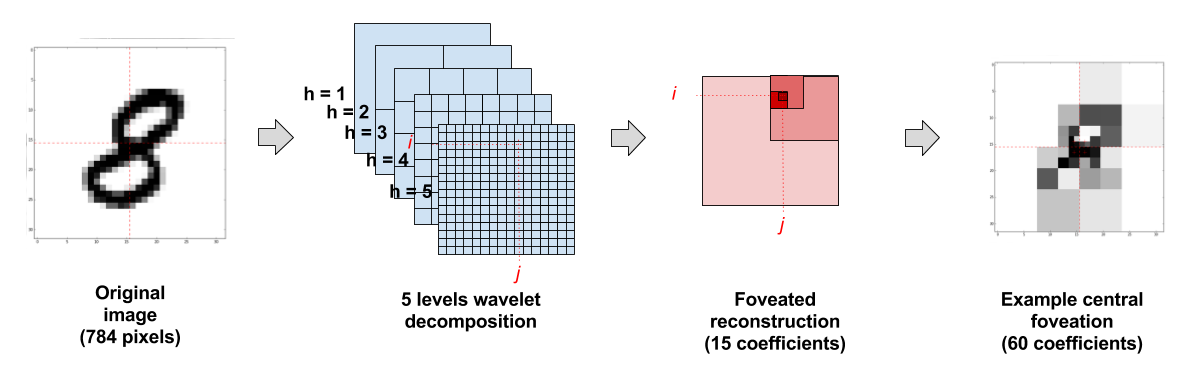
\includegraphics[width = \linewidth]{img/ICLR-foveated-model.png} 
	}
	\caption{Foveated image construction}\label{fig:foveated}
\end{figure}

The baseline foveated vision model we propose relies first on learning local foveated views on images. Foveated image decomposition is rarely proposed in literature for machine learning purposes, at the exception of Simoncelli's group that has developed a framework to process centrally-magnified images in a bio-realistic fashion (see \cite{freeman2011metamers} and \cite{Deza2016piranhas}). For simplicity and consistency purposes, we restrain here the foveal transformation to its core algorithmic elements, i.e. the compression of an image according to a particular spatial focus. The essential properties of foveated images is that they retain high spatial frequency information at the center an keep only low-frequency information at the periphery. Our foveal image compression rests on a 2D wavelet decomposition of images according to the Haar wavelets dictionary. Taking the example of the MNIST database, we first transform the original images according to a 5-levels wavelet decomposition (see figure \ref{fig:foveated}). We then define a viewpoint $u$ as a set of 3 coordinates $(i,j,h)$, with $i$ the row index, $j$ the column index and $h$ the spatial scale. Each $u$ may correspond with a visual field made of three of wavelet coefficients $\boldsymbol{x}_{i,j,h} \in \mathbb{R}^3$, obtained from an horizontal, a vertical and an oblique filter at location $(i,j)$ and scale $h$.  The multiscale visual information $\boldsymbol{x}_{i,j} \in \mathbb{R}^{15}$ available at coordinates $(i,j)$ corresponds to a set of 5 coefficient triplets, namely $\boldsymbol{x}_{i,j}=\{\boldsymbol{x}_{i,j,5}, \boldsymbol{x}_{\lfloor i/2\rfloor,\lfloor j/2\rfloor,4}, \boldsymbol{x}_{\lfloor i/4\rfloor,\lfloor j/4\rfloor,3}, \boldsymbol{x}_{\lfloor i/8\rfloor,\lfloor j/8\rfloor, 2}, \boldsymbol{x}_{\lfloor i/16\rfloor,\lfloor j/16\rfloor, 1}\}$ (see figure \ref{fig:foveated}), so that each multiscale visual field owns 15 coefficients (as opposed to 784 pixels in the original image).
The rightmost image in figure \ref{fig:foveated} displays a reconstructed image from the 4 central viewpoints at coordinates (7, 7), (7, 8) (8, 7) and (8, 8).

A weak generative model is learned for each $u = (i,j,h)$ (making a total of 266 weak models) over 55,000 examples of the MNIST database. For each category $z$ and each position $u$, a generative model is built over parameter set $\Theta_{z,u} = (\rho_{z,u}, \boldsymbol{\mu}_{z,u}, \boldsymbol{\Sigma}_{z,u})$, so that $\forall z,u, \tilde{\boldsymbol{x}}_{z,u} \sim \mathcal{B}(\rho_{z,u}) \times \mathcal{N}(\boldsymbol{\mu}_{z,u}, \boldsymbol{\Sigma}_{z,u})$ with $\mathcal{B}$ a Bernouilli distribution and $\mathcal{N}$ a multivariate Gaussian. The Bernouilli reports the case where the coefficient triplet is null in the considered portion of the image (which is quite common in the peripheral portions of the image), which results in discarding the corresponding triplet from the Gaussian moments calculation. Each resulting weak generative model $p(.|z,u)$ is a mixture of Bernouilli-gated Gaussians over the 10 MNIST labels. For the generative model, a posterior can here be calculated explicitly using Bayes rule, i.e. $q(.|\boldsymbol{x},u) = \text{softmax} \log p(\boldsymbol{x}|.,u)$.

The saccade exploration algorithm is an adaptation of algorithm \ref{algo:saccade}. The process starts from a loose assumption based on reading the baseline lower-level coefficient of the image, from which an initial guess $\rho_0$ is formed. Then, each follow-up saccade is calculated on the basis of final coordinates $(i,j) \in [0,..,15]^2$, so that the posterior calculation is based on several coefficient triplets. After selecting $(i,j)$, all the corresponding coordinate triplets $(h,i,j)$ are discarded from $\mathcal{U}$ and can not be reused for upcoming posterior estimation (for the final posterior estimate may be consistent with a uniform scan over the wavelet coefficients). 

\begin{figure}[t!]
	\centerline{
		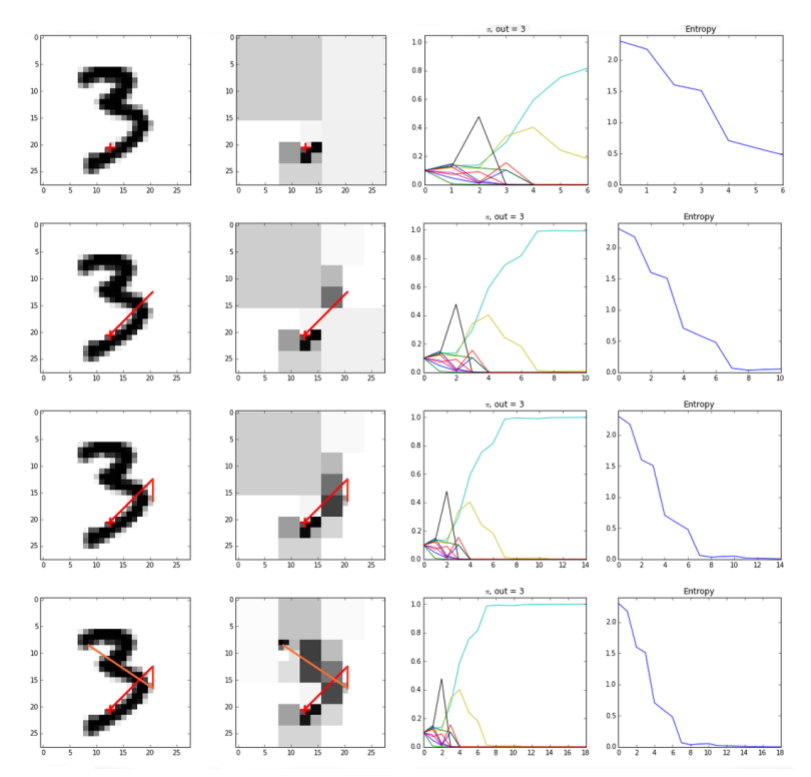
\includegraphics[width = .7\linewidth]{img/ICLR-foveated-saccades.png} 
	}
	\caption{Image exploration through saccades in the foveated vision model. The left column gives the successive saccades position over the original image. The second column shows the progressive image reconstruction from the coefficients gathered from the saccadic exploration. The third column shows the evolution of the posterior distribution in function of the number of wavelet coefficients triplets read out. The last columns provides the update of the entropy of the posterior distribution}\label{fig:foveated-saccades}
\end{figure}


An example of such saccadic image exploration is presented in figure \ref{fig:foveated-saccades}.
The first row shows the state of the process after one saccade. If we look at the central right figure, we see the accumulation of evidence over the scale sub-steps. There is a total of six sub-steps (not including the uniform basis step), over which a posterior is formed on the basis of 15 wavelet coefficients (plus a baseline wavelet coefficient summing all the pixels), that provide a recognition probability around 80\% for the category 3 (that is correct here). The next saccade (second row) heads toward a region of the image that is expected to help confirm the guess, which is the case for the recognition climbs up to about 99\%. The next saccade (third row) allows to reach 99.9\% in favor of class 3, and the final saccade (last row) allows to reach the threshold, set at $H_\text{ref} = 1e^{-5}$ for the entropy.   

The model provides apparently realistic saccades, for they cover the full range of the image and tend to point over regions that contain class-characteristic pixels. The image reconstruction after 4 saccades allows to visually recognize a "fuzzy" three, while it would not have been the case if the saccades had been chosen at random.
The observed trajectory illustrates the \emph{guess confirmation} logic that is behind the active vision framework. Every saccade heads toward a region that is supposed to confirm the current hypothesis. This confirmation bias appears counter-intuitive at first sight, for some would expect the eye to head toward places that may \emph{infirm} the assumption (to challenge the current hypothesis). This is actually not the case for the class-confirming regions are more scarce than the class-infirming regions, so that heading toward a class-confirming region may bring more information in the case it would, by surprise, invalidate the initial assumption.

A strong aspect of the model is the search for an optimal image processing compression, that is reflected in the number of wavelet coefficients used in the reconstruction. The median number of saccades is between 10 and 15 in our setting, corresponding to a compression rate of about 85 \%. It can be more if the threshold is more optimistic, and less if it is more conservative. The number of saccades is representative of the recognition difficulty. Few saccades reflect a ``peace-of-cake'' recognition, while many saccades reflect a hard-to-reach recognition.  

\begin{figure}[t!]
	\centerline{
		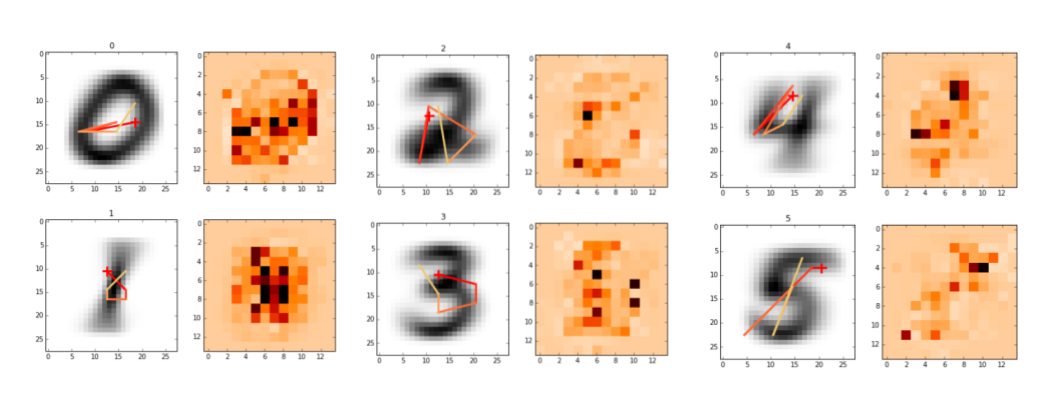
\includegraphics[width = \linewidth]{img/ICLR-saliency-maps.png} 
	}
	\caption{Saliency maps inferred from the model and corresponding saccades prototypic trajectories for the six first categories.}\label{fig:saliency-maps}
\end{figure}

With a posterior approaching $1 - 1e^{-5}$, the model is overconfident in its own predictions which introduces a confirmation bias that tends to harm the final recognition rate of the model (which is here around 92\% classification accuracy). It must be noticed however that the confirmation bias is probably a more general feature of the active inference framework that should be specifically addressed. For there is no free lunch, it corresponds to the "price to pay" for reducing the observation range of the image at the risk of potentially neglecting critical information. 

Another follow-up aspect is the bad scaling of the full predictive model when large images are considered. A critical component of the predictive model is the two-steps ahead prediction that is necessary for the future posterior estimate. It seems in practice unrealistic to make prediction over the whole action set to foresee every possible consequences of every action. Rather a parametrized policy would be much preferable, allowing for a single draw over the action set.
Luckily, this parametrized policy is relatively straightforward to compute in advance, given a generative model $p$. Taking $z_0$ as an initial guess, if we note $\tilde{\boldsymbol{x}}_{u,z_0}$ the visual field generative prediction when the object $z_0$ is assumed under visual orientation $u$, then, assuming a uniform prior over the external states, the process-independent look-ahead posterior is~:
\begin{align}
%\forall u, \rho(.)|_{u, z_0} = \text{softmax} \left[\log P(\tilde{\boldsymbol{x}}_{u, z_0}|.,u) + \log P(.|u, z_0) + \rho_0[z_0]\right]
\rho(.)|_{u, z_0} = \text{softmax} [\log p(\tilde{\boldsymbol{x}}_{u, z_0}|.,u)]
\end{align}
%Then, , one obtains $\rho(.)|_{u, z_0} = \text{softmax} [\log P(\tilde{\boldsymbol{x}}_{u, z_0}|.,u)]$ 
providing at each $(u, z_0)$ an offline pre-processing of the predictive computations, namely $\rho(z_0)|_{u, z_0}$. Those offline computations provide, for each guess $z_0$, a saliency map over the $u$'s. {\color{blue} Each saliency map then provides an optimal pathway through the image, that, given a certain assumption $z$, follows an evidence-decreasing sequence of viewpoints regarding $z$'s confirmation.}  

Examples of such saliency maps are provided in figure \ref{fig:saliency-maps}, for categories 0 to 5. The saliency maps allow to analyze in more detail the class-specific locations (that appear brownish) as opposed to the class-unspecific locations (pale orange to white). First to be noticed is the relative scarceness of the class-specific locations. Those "evidence providing" locations appear, as expected, mutually exclusive from category to category. A small set of saccades is expected to provide most of the classification information while the rest of the image is putatively uninformative (or even counter informative if whitish). A second aspect is that the class-relevant locations are all located in the central part of the images, so there is very few chance for the saccades to explore the periphery of the image where little information is expected to be found. This indicates that the model has captured the essential concentration of class-relevant information in the central part of the images for that particular training set.

\section{Outlook and perspectives}

We developed a comprehensive description of the active inference framework, as proposed by \cite{friston2010free} and \cite{friston2012perceptions}, under a machine-learning compliant perspective. Stemming from a biological inspiration and the auto-encoding principles, we develop a sketch of a cognitive architecture that should provide ways to implement \emph{estimation-oriented} control policies.
This may be particularly useful for developing active information search in the case high dimensionality input data.
The pros and cons of the approach are reviewed in details, showing interesting promises in term of computation compression, but also putative risks of a confirmation bias that may degrade the recognition performance if the model is too optimistic about its own predictions. The presented formalism is fully compliant with the auto-encoding framework and would deserve further developments with deep variational auto-encoders \cite{makhzani2015adversarial}.

\bibliography{biblio}
\bibliographystyle{iclr2017_conference}

\end{document}
